%! Author = Vova
%! Date = 28.07.2021

% Preamble
\documentclass[11pt]{article}

% Packages
\usepackage{amsmath}
\usepackage{hyperref}
\usepackage{polyglossia}
\usepackage{fontspec}
\usepackage{graphicx}
\usepackage{babel,blindtext}
\usepackage{subfig}
\usepackage{iftex}
\usepackage{xcolor}
\usepackage{amssymb}
\usepackage{adjustbox}
\usepackage[normalem]{ulem}
\usepackage{amsfonts}
\usepackage{placeins}
\usepackage{listings}

\lstset{basicstyle=\ttfamily,keywordstyle=\underbar,morekeywords={plot,solve,optimize,for,in,minorant}}

% Language and Font settings

% Kurale
% New Standard Old
\setdefaultlanguage{russian}
\setmainfont[Ligatures=TeX]{Kurale}
\newfontfamily\cyrillicfont{Kurale}
\newfontfamily\cyrillicfontsf{Kurale}

% Author, date
\title{Описание Математического Бота}
\author{Латыпов Владимир Витальевич}
\date{\today}

% Graphics settings
\graphicspath{{../images/}}



% Document
\begin{document}

    \maketitle
    \newpage

    \tableofcontents
    \newpage


    \section{Формулировка задачи}\label{sec:formulating-task}
    Математический бот — это набор инструментов для работы с математическими сущностями через интерфейс привычных нам социальных сетей.
    В отличие от WolframAlpha, бот специализируется на оптимизации многомерных функций и численном решении уравнений с большим количеством переменных
    (проверено, что с этим бот справляется лучше).

    Чтобы пообщаться с ботом, достаточно написать в сообщения группы: \url{https://vk.com/true_mathbot}.

    Технически бот состоит из двух частей:
    \begin{itemize}
        \item Условный «front-end» — программа (написана на python), которая через vk\_api выполняет коммуникативную функцию, то есть общается с пользователем и,
        когда требуется, вызывает основной блок.
        \item А именно — «back-end» интерфейс, который написан на C++ и компилируется в полноценное консольное приложение.
        Он и занимается оптимизацией функций, решениями уравнений и т.д.
    \end{itemize}

    Поэтому больший интерес, конечно, представляет back-end часть.
    Используется авторская библиотека для разбора математических выражений, умеющая в частности аналитически находить производные.

    Для высококачественной оптимизации функции используется комбинация различных методов с помощью дерева оптимизации.
    Вот эти методы:
    \begin{itemize}
        \item Генетический алгоритм
        \item Алгоритм симуляции отжига
        \item Градиентный спуск
        \item Метод Ньютона
    \end{itemize}
    Последние два используют вычисление градиента и вторых производных, что реализуется с помощью автоматической
    генерации дерева вычислений для производных.


    \section{Обзор}\label{sec:overview}

    Бот умеет:
    \begin{itemize}
        \item Оптимизировать функции
        \item Решать уравнения
        \item Строить графики
    \end{itemize}

    Третий режим добавлен для удобства — чтобы рассматривать функции (правда, пока только 2-х мерные),
    не выходя из диалога с ботом.

    Во всех случаях вводится математическое выражение и, возможно, дополнительные параметры.
    Предусмотренно два варианта введения запросов боту:
    \begin{itemize}
        \item Через коммуникацию: от пользователя требуется читать сообщения бота, предложенные ответы, знакомясь с интерфейсом бота,
              и, отвечать на них (зачастую достаточно выбрать вариант из предложенных).
              Этот вариант подходит для людей, которые только знакомятся с возможностями бота.
        \item Quick Input Mode (QIM).
              Если пользователь точно знает, что ему нужно и что значат аргументы, для него целесообразно использовать эту возможность.
              Вся информация для запроса передаётся одним сообщением, содержащим корректрую команду QIM.

        Типичный запрос выглядит так (переносы строки не важны): \newline

        \begin{lstlisting}[label={lst:QIM-example}]
            optimize x + y^2 - 1000.5
            for x in [-10; 100],
            y in (10.3e-100, 123)
            | minorant 10
        \end{lstlisting}

    \end{itemize}

    Подробнее об интерфейсе можно прочитать в Инструкции (ВСТАВИТЬ ССЫЛКУ!).


    В отличие от других подобных инструментов, бот предоставляет дружелюбный интерфейс: если пользователь что-то некорректно указал,
    бот известит его об этом.
    Однако иногда бот проверяет характер: например, ему не очень нравится, когда много раз неправильно указывают аргумент или
    когда пишут с маленькой буквы.

    \section{Технические подробности}

    Исходный ход backend-части (написан на C++) находится в github-репозитории \url{https://github.com/donRumata03/MathBotBackend}.
    Больша́я часть функционала реализована не в этом репозитории непосредственно, а вынесена в другие.
    Так, для общих целей используется моя библиотека pythonic: \url{https://github.com/donRumata03/pythonic}
    Для алгоритмов оптимизации — моя библиотека PowerfulGA: \url{https://github.com/donRumata03/PowerfulGA}

    А разбор выражений и аналитическая работа с ними осуществляется в репозитории \url{https://github.com/donRumata03/ExpressionParsing}
    (Подробнее про эту часть проекта — в секции~\ref{subsec:expression-parsing}).

    Код коммуникативной части можно найти здесь: \url{https://github.com/donRumata03/MathBotFrontend}.

    \section{Описание алгоритма в общих чертах}

    \subsection{Разбор выражений}\label{subsec:expression-parsing}
    Чтобы работать с уравнением или функицей, нужно для начала распарсить строку и представить в удобном для компьютера виде.
    В данном случае — это дерево вычислений (каждый узел — это либо числовое или переменное значение, либо операция, тогда узлы-дети содержат информацию об аргументах этой операции).
    % дерево не обязательно бинарное — у некоторых функций может быть больше двух аргументов

    Для получения дерева используется авторский алгоритм.
    У бота может быть своя специфика формата входных данных, поэтому использовать стороннюю библиотеку для этих целей — плохая идея.

    \subsubsection{Вычисление производной}

    Для некоторых алгоритмов нужно вычисление производной.
    С этой целью предусмотрена функция генерации производной по нужной переменной, метод дифференцирования - самый стандартный.
    Например, для степенной функции:
    \begin{figure}[h]
        \centering
        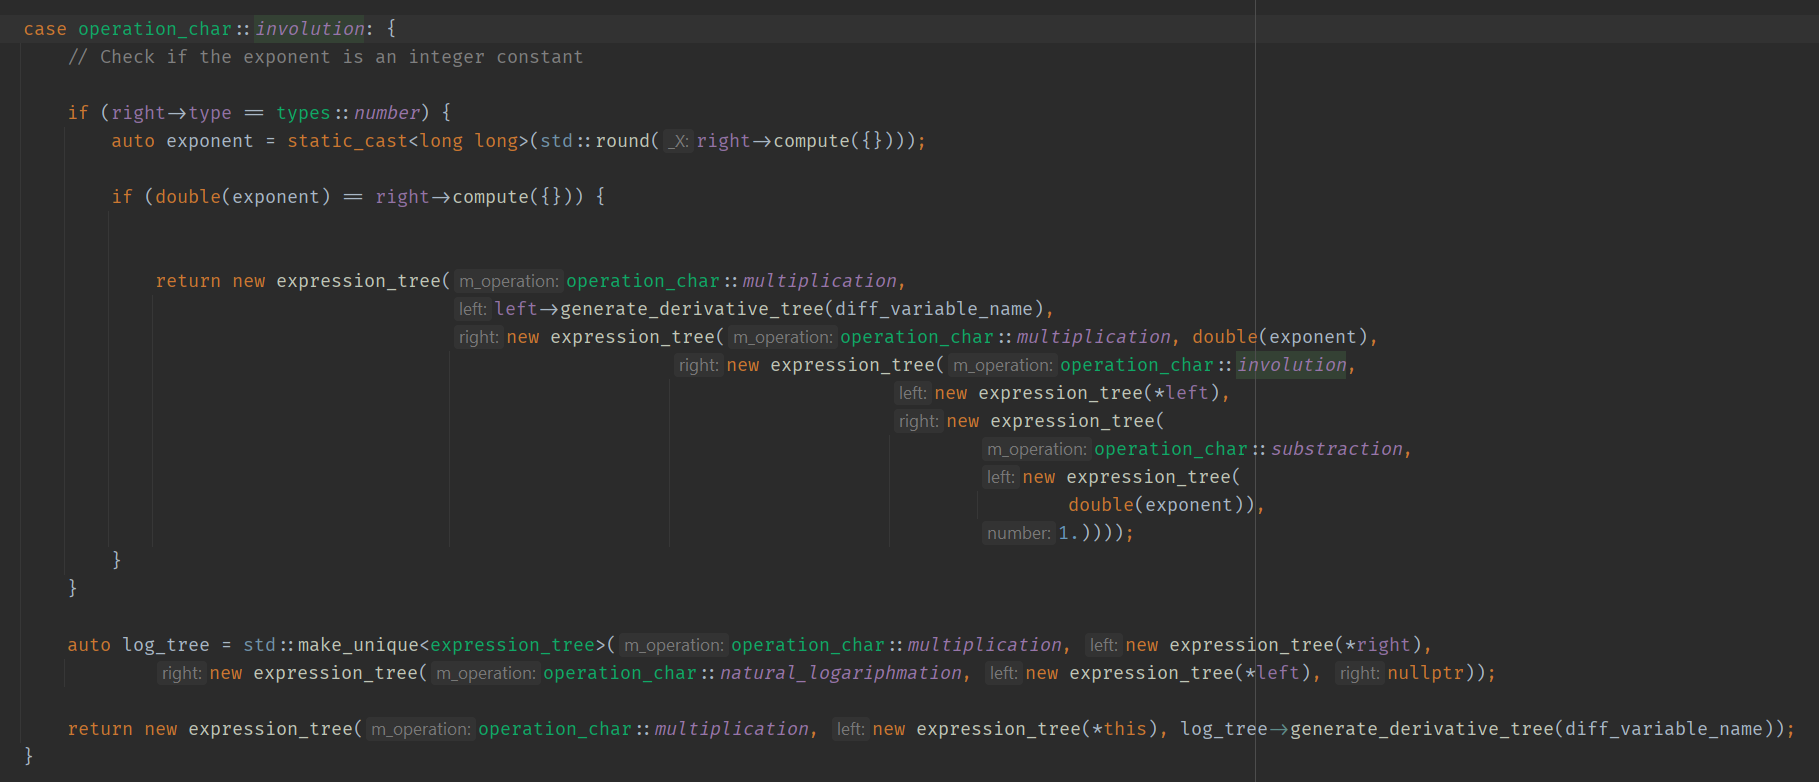
\includegraphics[width=0.7\textwidth]{involution_derivative.png}
        \label{fig:involution-derivative}
    \end{figure}
    \FloatBarrier

    Для «не дифференцируемых в каких-то точках функций», например,
    модуля или максимума нескольких других функций было решено находить всё равно заявлять возможность нахождения производной,
    и выдавать, например, ноль в месте перелома, надеясь, на то,
    что вероятность попасть в одну конкретную точку бесконечно мала не только в идеальном случае.

    \subsubsection{Оптимизация вычислений}
    Часто бывает так, что какую-то часть функции можно посчитать сразу, не зная значения переменных.
    Это позволило бы произвести некоторую часть вычислений один, а не огромное количество раз, что существенно ускоряет процесс.

    Такая возможность реализована.
    Более того, происходит сортировка операндов в ряде одинаковых и (в некоторых случаях) в операциях с одинаковым приоритетом
    по признаку вычислимости на этапе «компиляции» дерева.
    Это делается, чтобы лучше оптимизировать подобные выражения:

    $10 + x + 11 * exp(3) \longrightarrow (10 + 11 * exp(3)) + x \longrightarrow (\approx 230.94) + x$

    У некоторых операций есть нейтральные элементы.
    Значение элемента не меняется после проведения с ним операции с этим элементом,
    но время на такую операцию тратится.
    Например, $x + 0 = x$, $x^1 = x$ и т.д.
    Поэтому сразу после компиляции эти операции «are optimized out».


    \subsection{Дерево алгоритмов оптимизации}\label{subsec:opt-algo-tree}

    \subsubsection{Идея}\label{subsubsec:opt-tree-idea}
    Комбинируя разные алгоритмы, можно получить существенно более хороший результат, чем при запуске их по отдельности.
    Но важно понимать, в какой последовательности их лучше запускать.

    Здесь нужно понимать, что, проектируя алгоритм оптимизации, приходится выбирать между скоростью
    сходимости и вероятностью попасть в локальный оптимум, не найдя то, что искали (конечно, это упрощённая картина, но полезно посмотреть под таким углом).

    \begin{figure}[h]
        \centering
        
\includegraphics[width=0.6\textwidth]{balance.jpg}
        \label{fig:perfect-balance}
    \end{figure}
    \FloatBarrier

    Умение избегать локальных оптимумов ради нахождения глобальных назовём \underline{глобальностью} алгоритма.

    Для понимания, как комбинировать алгоритмы, полезна идея: когда алгоритм с высокой глобальностью уже нашёл некую окрестность, в которой,
    по его мнению, находится оптимум, имеет смысл передать его результат в более локальный алгоритм,
    чтобы увеличить скорость и точность без потери этой окрестности.

    Реализованные алгоритмы, которые могут быть полезны:
    \begin{itemize}
        \item Генетический алгоритм
        \item Алгоритм симуляции отжига
        \item Градиентный спуск
        \item Метод Ньютона
    \end{itemize}

    Алгоритмы расположены в порядке увеличения скорости сходимости и уменьшения глобальности.
    (Метод Ньютона можно назвать менее глобальным, чем градиентный спуск, так как он ищет не «ближайший» минимум,
    а любой «ближайший» экстремум (корень производной в данном случае))

    Причём у некоторых алгоритмов есть разные гиперпараметры, которые также регулируют этот скорость сходимости.
    Проанализировав всё это, я пришёл к выводу, что целесообразно подключение алгоритмов друг к другу примерно так, как это описано
    в следующем разделе.

    \subsubsection{Схема дерева}

    На схеме используются такие обозначения алгоритмов:
    \begin{itemize}
        \item GA — Genetic Algorithm (генетический алгоритм)
        \item Annealing — Метод симуляции отжига
        \item GD — Gradient Descent (градиентный спуск)
        \item Newton — метод Ньютона
    \end{itemize}

    \begin{figure}[h]
        \centering
        \adjincludegraphics[width=\textwidth, clip, trim={0.0\width} {0.35\height} {0.0\width} {0.0\height}]{OptTree_scheme.pdf}
        \caption{Схема дерева оптимизации}
        \label{fig:opt-tree}
    \end{figure}
    \FloatBarrier
    (Первому слою не даётся никакого начального приближения)

    Как видно из схемы, предполагается параллельное и последовательное соединение блоков.

    При параллельном каждому child'у на вход даётся одно и то же начальное приближение (или его отсутствие, если первый слой),
    а выход параллельного блока — лучший из результатов его «child»-ов.

    При параллельном — каждому следующему на вход даётся лучший из выходов всех предыдущих,
    а в качестве ответа также возвращается лучший из выходов child-ов.

    В последовательном контейнере могут лежать как «голые» блоки, так и целые параллельные контейнеры.
    С параллельным блоком — аналогично.

    Структура дерева задаётся через .json файл
    (пока что используется один и тот же файл для разных пользователей, но, возможно,
    в будущем имеет смысл изменять файл в зависимости, например, от наличия VIP-статуса у пользователя или от сложности его задачи).

    \begin{figure}[h]
        \centering
        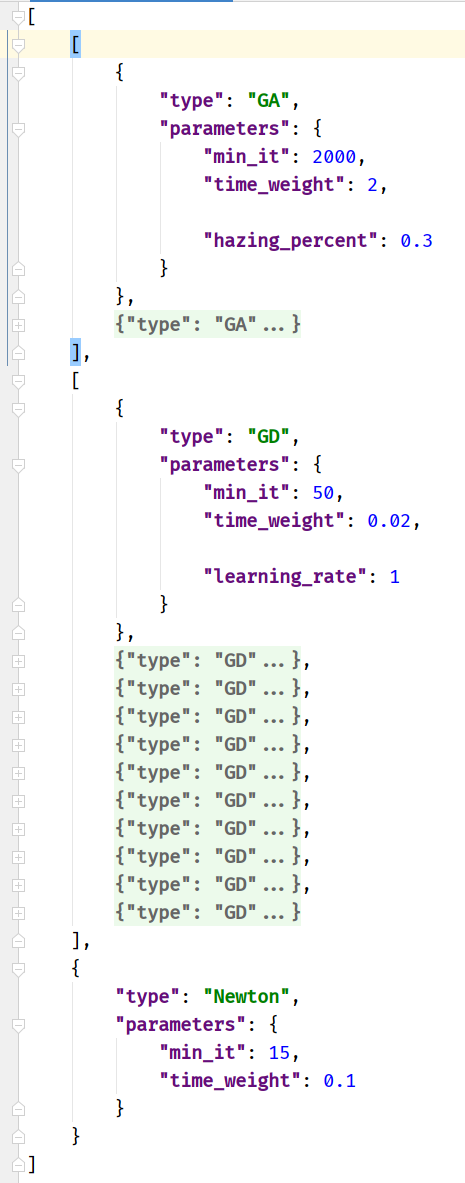
\includegraphics[height=0.4\textheight]{opt-tree-json.png}
        \label{fig:opt-tree-config}
        \caption{Пример конфигурационного файла}
    \end{figure}
    \FloatBarrier

    Также важная часть схемы — индивидуальные параметры блоков.
    Параметры \{ min\_it, time\_weight \} есть у каждого блока вне зависимости от его типа.

    Есть и типоспецифичные параметры.
    Например, hazing\_percent для ГА и learning\_rate для градиентного спуска.
    Как видно из схемы, на соответствующих слоях расположено несколько алгоритмов этих типов с разными значениями этих параметров.
    Такая конфигурация нужна потому, что для разных функций лучше будут работать вариации с разными параметрами.

    Например, learning\_rate-ы у разных экземпляров GD распределены равномерно в логарифмическом пространстве, чтобы покрыть
    как можно больший спектр разнообразных функций.

    \subsubsection{Распределение вычислительного ресурса}\label{subsubsec:resource-distribution}

    В случае МатБота результаты профайлинга подтверждают предположение о том, что бо́льшая часть вычислительного времени ($\gg 95\%$)
    используется именно для подсчёта функции ошибки, а не для операций с геномами.

    В условиях, когда выделенное количество вычислительных ресурсов может быть разным для разных людей и запросов,
    особенно остро встаёт вопрос о распределении этих вычислительных ресурсов.

    Изначально backend-части бота на вход поступает число — условно «целевое количество итераций».
    По сути это выделенное для работы время, рассчитанное в количестве вычислений функции ошибки.

    Это время было решено распределять пропорционально параметру time\_weight (но количество итераций ограничено снизу порогом min\_it).
    Но тут важно понимать, что это «время» — ещё не конечное значение итераций.

    Во-первых, в ГА непонятно, к чему применять слово «итерации» (см.~\ref{sec:ga-modifications}).

    Во-вторых, градиентный спуск и метод Ньютона используют первые и (Ньютон) частные производные,
    вычисление которых обычно сильно дольше, чем вычисление изначальной функции.

    Для сравнения — вот пример количеств операций для одной из тестовых функций:
    \begin{itemize}
        \item Сама функция: 22
        \item Первая производная: 123
        \item Вторая производная: 902
    \end{itemize}

    Размер дерева для 7-ой производной в памяти больше гигабайта, а попытка посчитать 8-ую привела необходимости насильственной перезагрузке компьютера.

    Кроме того, для этих алгоритмов нужно на каждой итерации вычислять значения этих производных по всем переменным, которых может быть немало.

    Поэтому для нахождения количества именно итераций нужно поделить выделенное время (в вычислениях обычной функции) на
    iteration\_cost для этого алгоритма.

    \subsection{Решение уравнений и построение графиков}
    Решение уравнения численными методами происходит с помощью оптимизации функции модуля разности частей с минорантой 0.

    График строится с использованием библиотеки matplotlib и загружается в ВК в виде картинки.
    Поддерживаются функции с прерывающейся на заданном промежутке областью определения (то есть те, вычисление которых кидает исключение).

    \section{Модификации в ГА}\label{sec:ga-modifications}
    Подробное описание ГА (в том числе — моей версии) можно найти в описании робота-художника в соответствующей секции.
    Здесь сосредоточусь на том, что относится конкретно к боту.

    В секции~\ref{subsubsec:resource-distribution} описано, как вычислительный ресурс распределяется между разными алгоритмами.
    Однако на том моменте, когда стало известно количество раз, сколько можно вычислить функцию ошибки вов время исполнения ГА,
    вопрос ещё не закрыт.

    Как известно, генетический алгоритм в каждую из $E$ «эпох» вычисляет функцию ошибки для $population\_size$ геномов.
    То есть суммарное количество вычислений: $computational\_resource = E \times population\_size$.

    Встаёт вопрос, какое соотношение значений $E$ и $population\_size$ обеспечивает наилучшую работу алгоритма.

    Я решил проверить это экспериментально.
    Изначальное предположение состоит в том, что разумно распределять ресурс так:

    \begin{equation}
        \begin{cases}
            E = computational\_resource^{epoch\_pow} \\
            population\_size = \frac{computational\_resource}{E} = computational\_resource^{1 - epoch\_pow}
        \end{cases}
    \end{equation}

    Вопрос был в том, какое $epoch\_pow$ выбрать.
    Для решения вопроса я выбрал функцию с более или менее сложным рельефом и для разного количества итераций
    построил графики зависимости достигаемого fitness (значения целевой fitness-функции) от $epoch\_pow$.

    Конечно, в целях помехоустойчивости для каждого $epoch\_pow$ делалось далеко не одно измерение.
    Важно оценивать не только минимальное, или только максимальное, или только некое среднее (иначе можно упустить важную информацию
    о недостатках или достоинствах того или иного $epoch\_pow$).

    Поэтому для комплексной оценки я посчитал «нечёткие» верхнюю и нижнюю границы множества значений fitness-а для нескольких попыток запуска.
    Под нечёткой нижней границей понимается такое число, которое бы оценило «почти худший случай работы алгоритма».
    С верхней границей — аналогично (почти лучший).

    Для их оценки я решил использовать вариацию среднего Колмогорова:
    \begin{equation}
        M(x_{1},\ldots ,x_{n})=\varphi ^{-1}\left({\frac {1}{n}}\sum _{k=1}^{n}\varphi (x_{k})\right)
    \end{equation}
    , где (в моём случае):

    для нижней границы $\varphi(x) = x^{-1.5}$ (это повышает чувствительность к малым значениям),
    для верхней границы $\varphi(x) = x^{2.5}$ (это повышает чувствительность к большим значениям).

    (альтернатива такой оценке — брать, например, результат алгоритмов для, например, 10-го и 90-го, процентилей,
    но этот метод хуже оценивает то, как именно распределены точки между ними и то,
    насколько сильно выбиваются верхние и нижние 10 процентов вверх и вниз по сравнению с остальными)

    Результаты таковы:
    \begin{figure}[h]
        \centering
        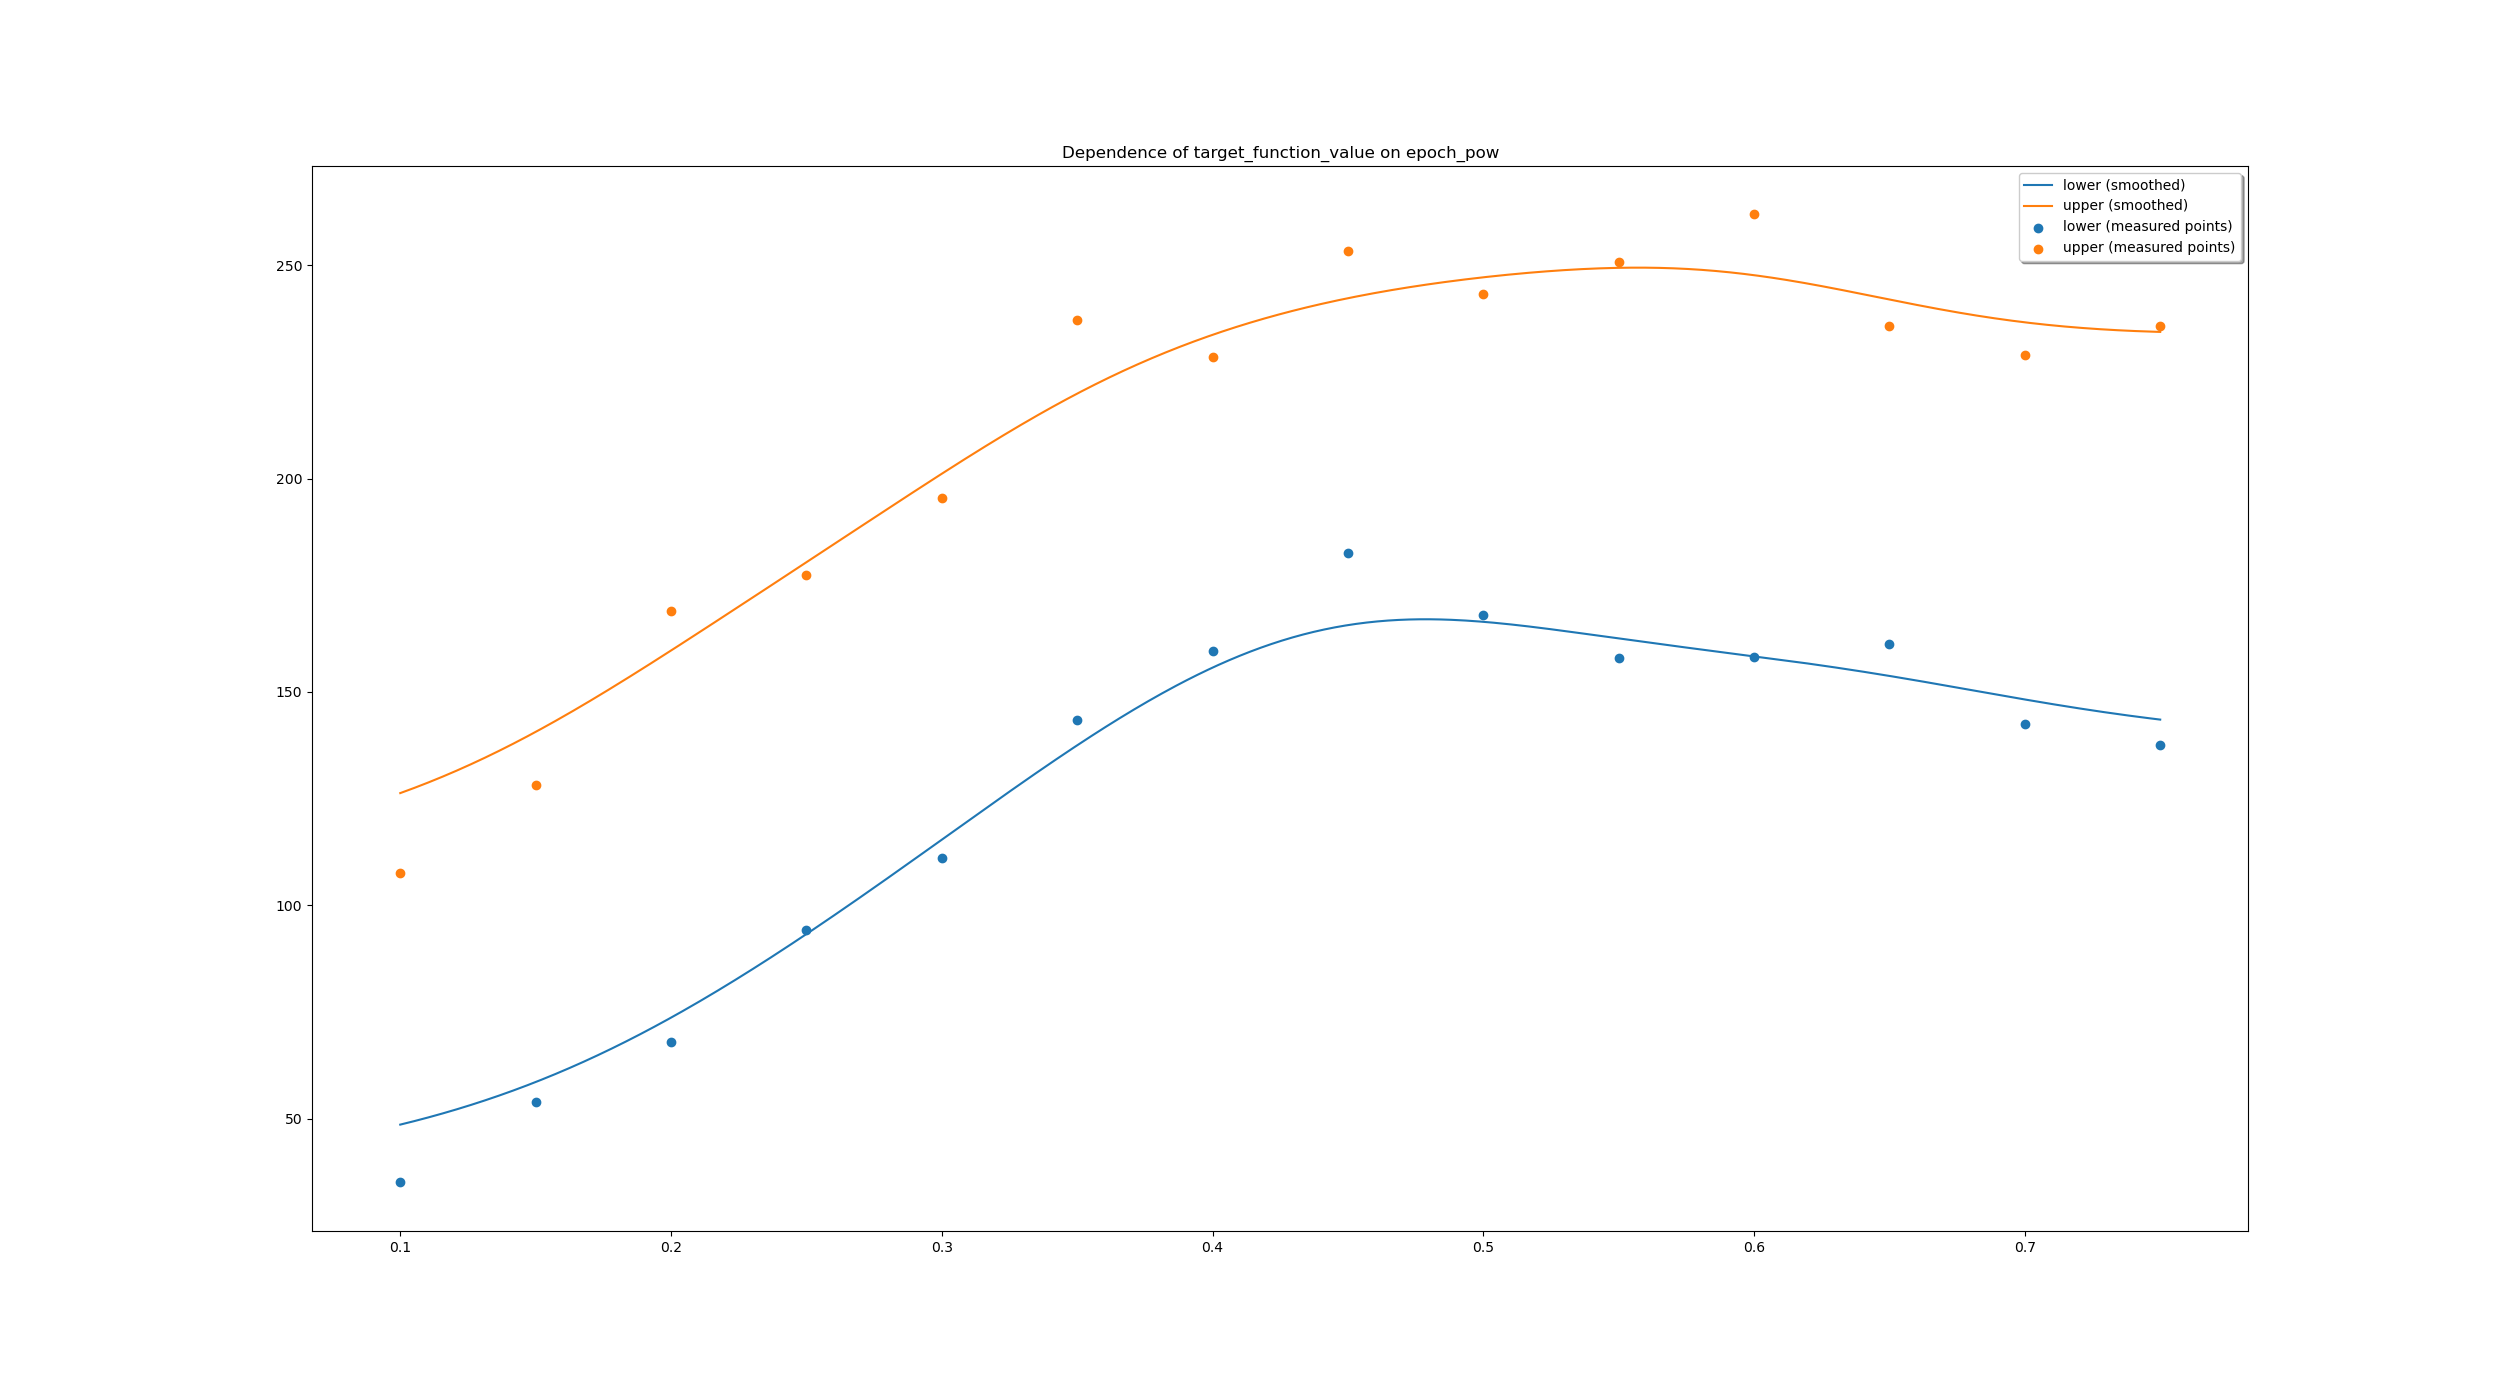
\includegraphics[width=0.75\textwidth]{exploring_optimal_epoch_pow_1000_iterations.png}
        \caption{График для 1'000 вычислений}
        \label{fig:epoch-pow-1000}
    \end{figure}
    \FloatBarrier

    \begin{figure}[h]
        \centering
        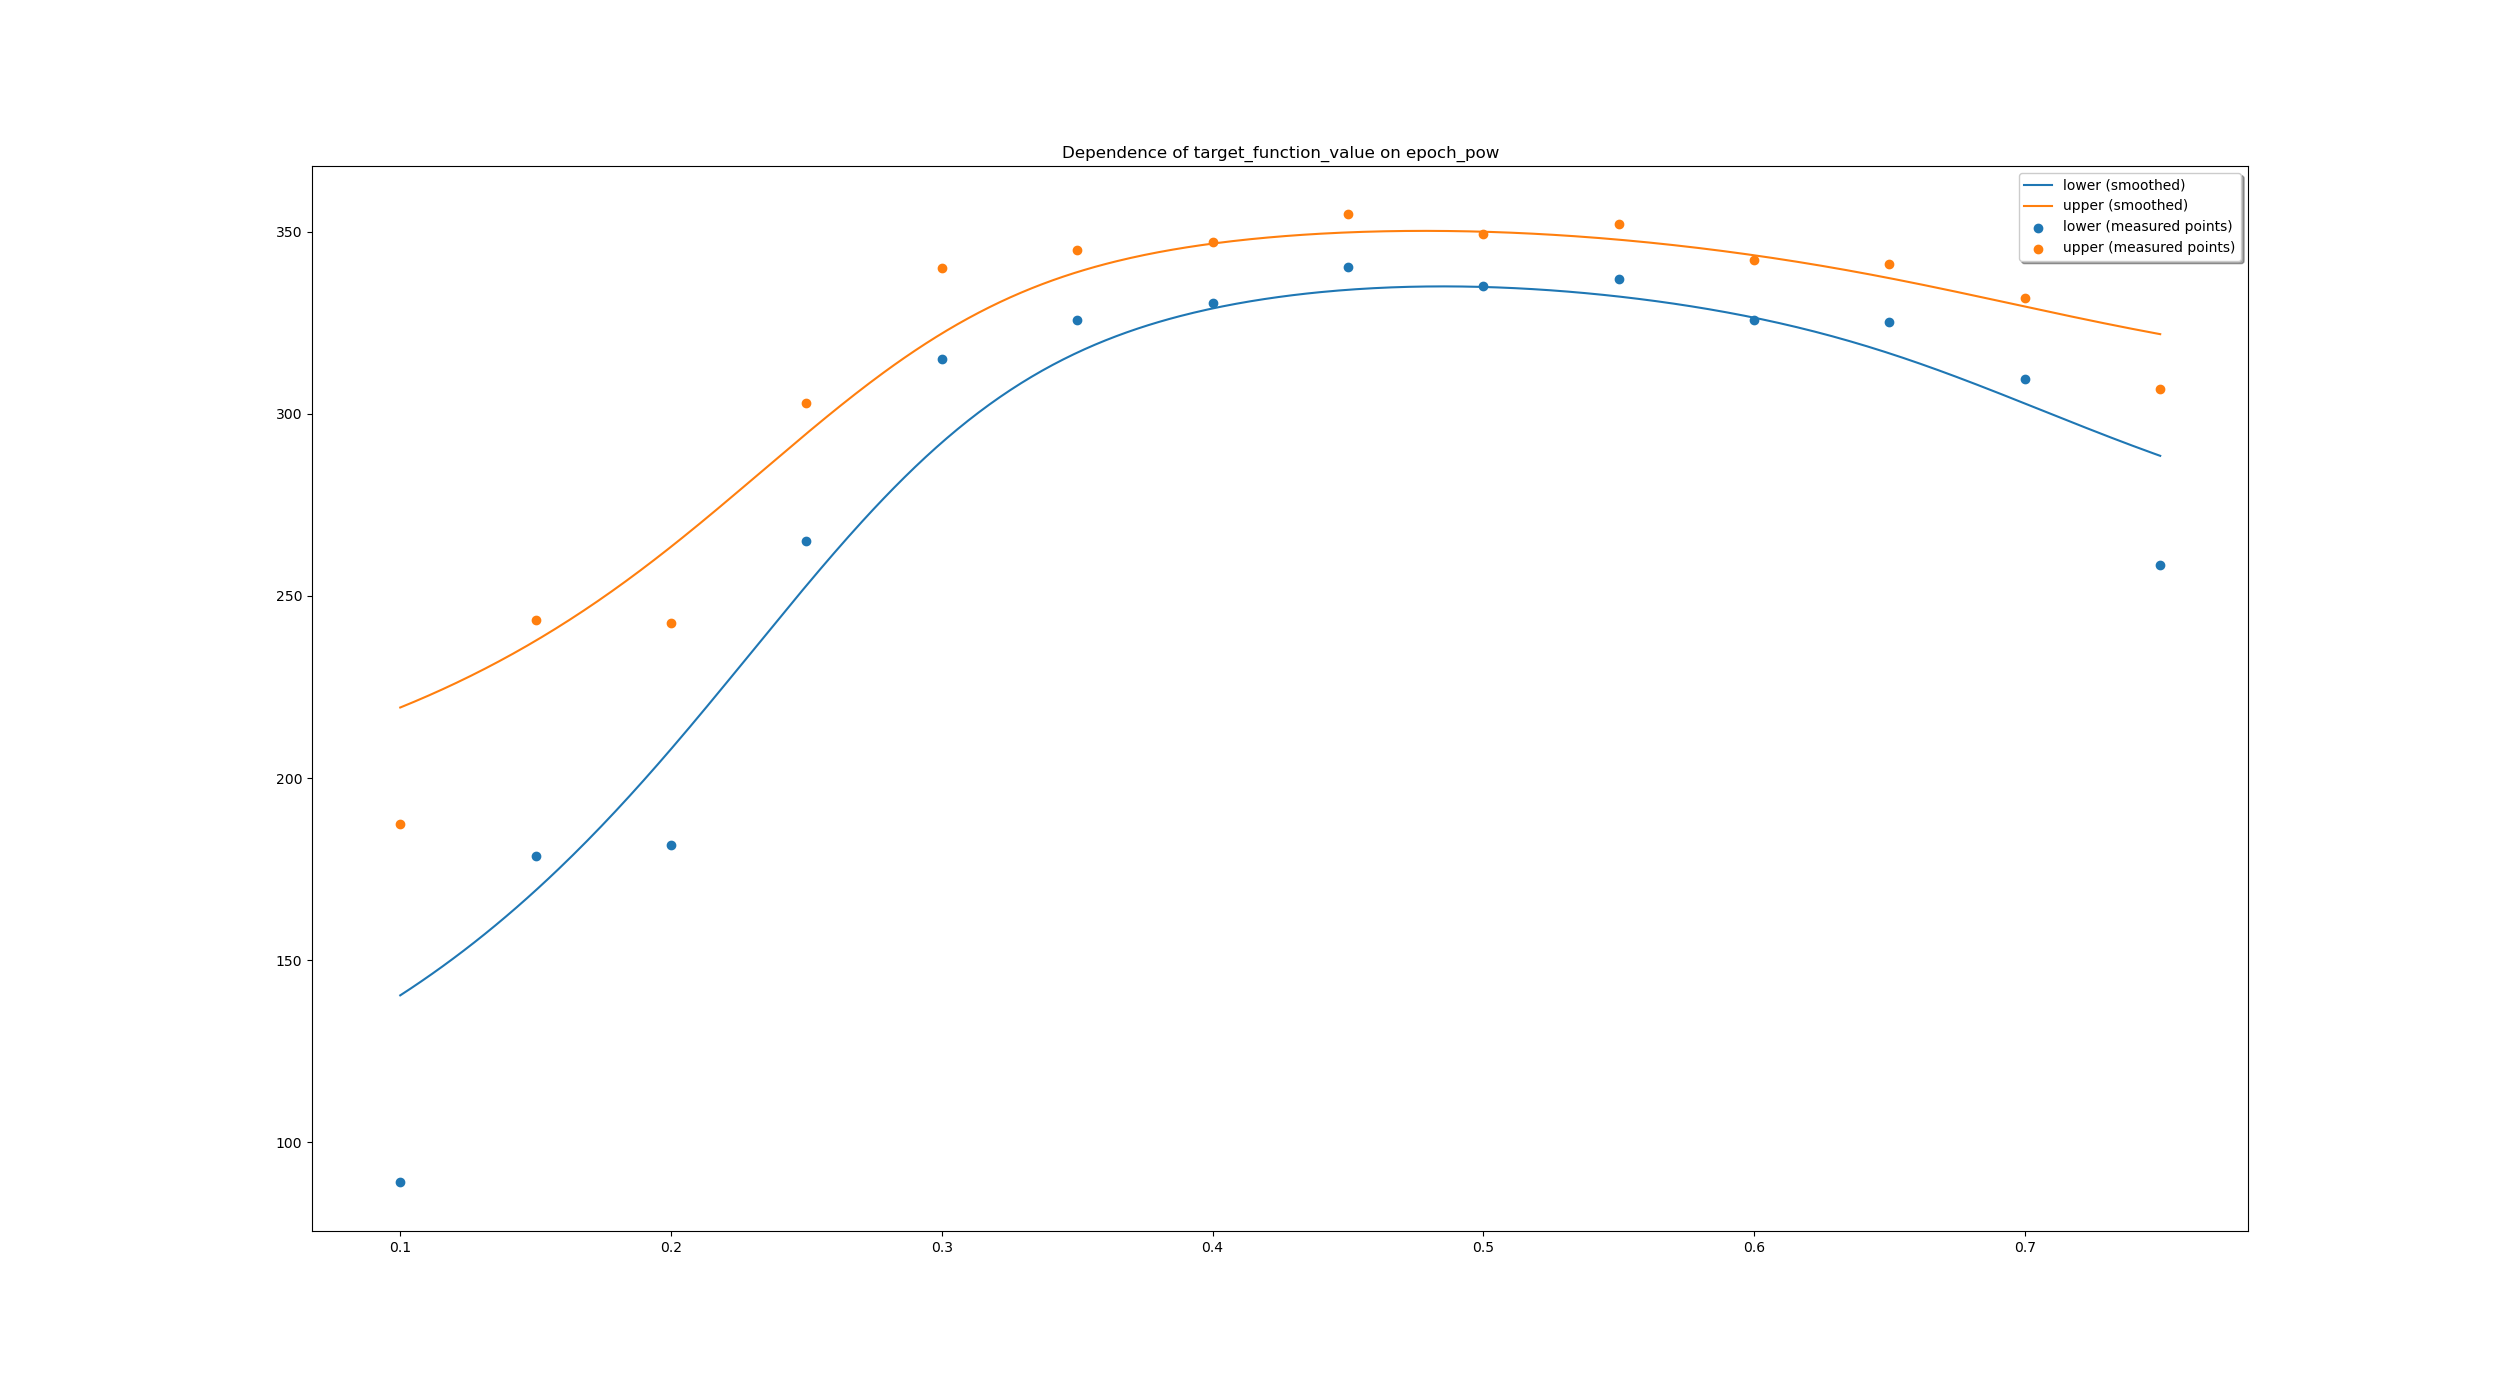
\includegraphics[width=0.75\textwidth]{exploring_optimal_epoch_pow_5000_iterations.png}
        \caption{График для 5'000 вычислений}
        \label{fig:epoch-pow-5000}
    \end{figure}
    \FloatBarrier

    \begin{figure}[h]
        \centering
        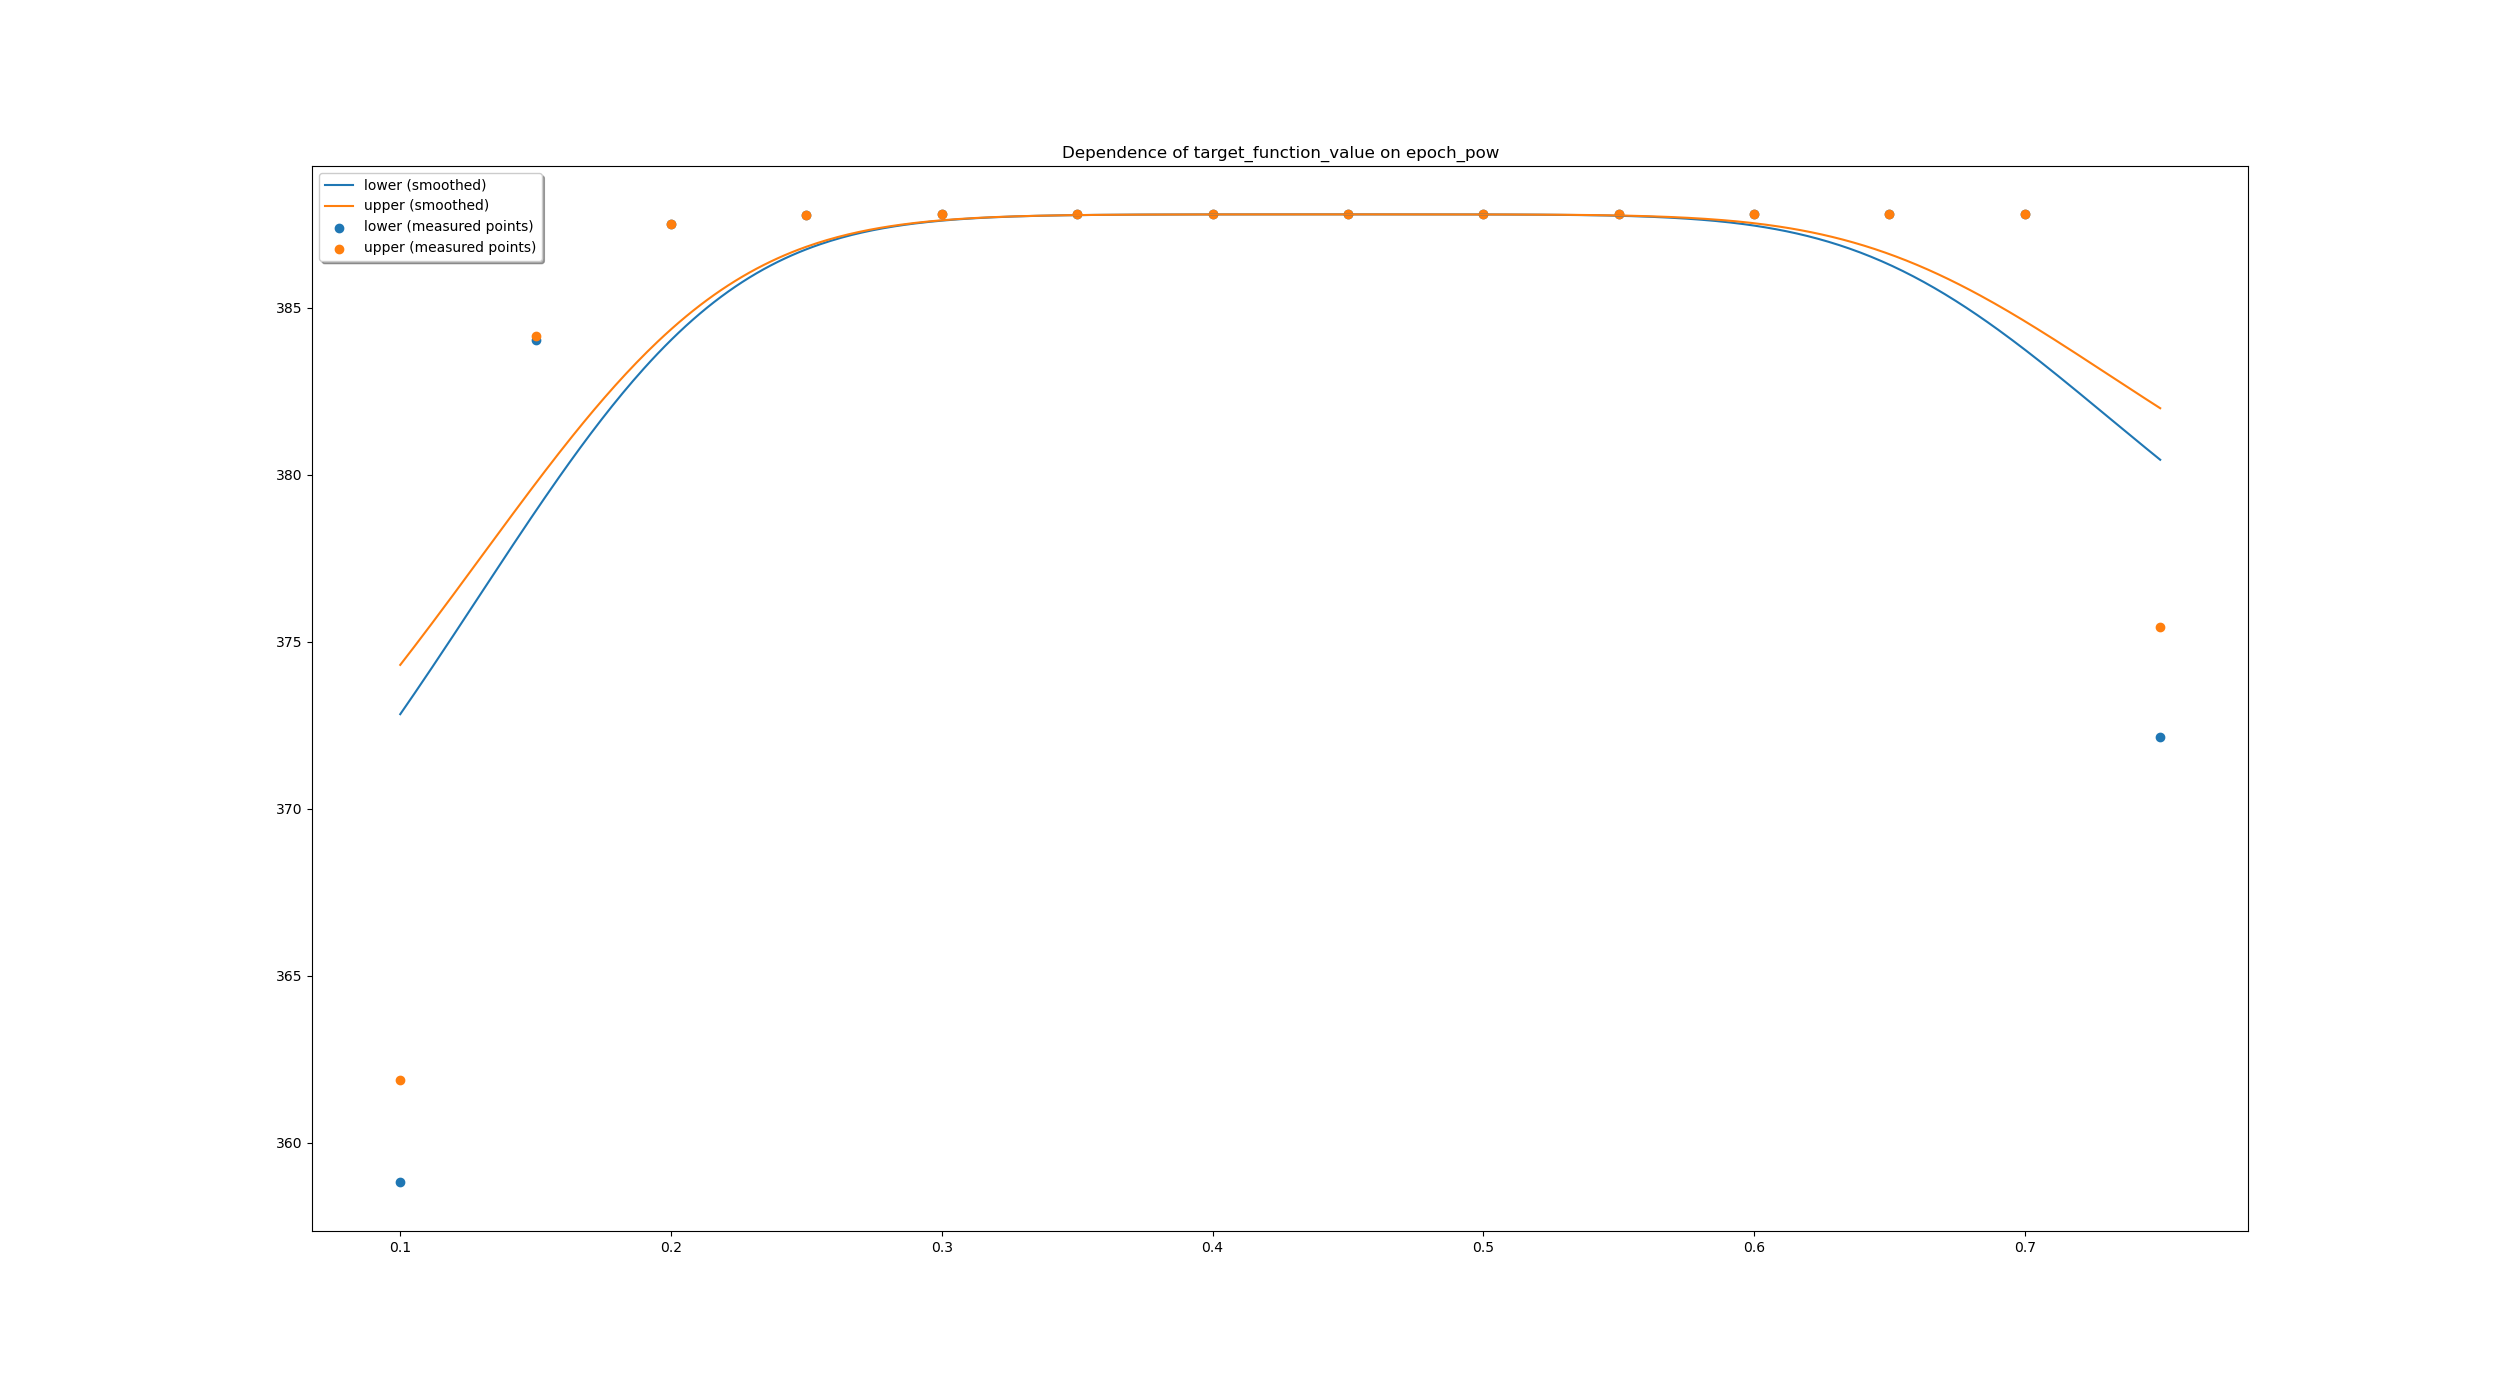
\includegraphics[width=0.75\textwidth]{exploring_optimal_epoch_pow_100000_iterations.png}
        \caption{График для 100'000 итераций}
        \label{fig:epoch-pow-100000}
    \end{figure}
    \FloatBarrier

    Проанализировав полученные данные, я пришёл к выводу, что лучше всего подходит значение $epoch\_pow \approx 0.45$

    \section{Тестирование}\label{sec:testing}
    Для тестирования бота использовались функции из основной таблицы этой статьи:
    \url{https://en.wikipedia.org/wiki/Test_functions_for_optimization}.

    На всех из них бот хорошо себя показал: нашёл требуемый оптимум.

    \section{Дальнейшее развитие}\label{sec:subsequent-development}

    Бот уже работает, с ним можно пообщаться, однако есть несколько напрашивающихся улучшений

    \subsection{Дополнительные алгоритмы оптимизации}
    В ближайшем будущем я планирую основательно подойти к изучению различных актуальных в наше время алгоритмов:
    как локальных, так и эволюционных, глобальных и обогатить дерево различными ветками, которые могут увеличить качество оптимизации.

    \subsection{Внедрение аналитических методов}
    Некоторые задачи не имеют аналитического решения или для его понимания нужно по-человечески думать (что бот всё-таки не может).
    Однако другие задачи — типовые — могут быть решены гораздо быстрее и точнее, если использовать наработки людей (например, квадратные или кубические уравнения).
    Свойства некоторых функций известны человечеству и без оптимизации, и это можно использовать в алгоритмах бота.
    Задачей или частью задачи бота может быть именно такая простая вещь.

    \subsection{Решение систем уравнений}
    Свести решение систем уравнений к оптимизационной задаче так же просто, как и сделать это для одного уравнения.
    Будет полезно добавить эту возможность.

    \subsection{Рендеринг формул в \LaTeX}
    В ближайшем будущем планируется реализовать рендеринг выражений в виде картинки.
    Это позволит, например, вывести вычисление производной в отдельный режим работы
    и выводить результат вычисления неопределённого интеграла некоторых функций (аналитический подсчёт интеграла ещё не реализован).

    \subsection{Построение многомерных графиков}
    При анализе функций, конечно, может быть полезно строить их графики, и очень неприятно,
    что большая часть инструментов построения графиков поддерживает только 2-х мерную плоскость,
    существенно реже — трёхмерные.
    Я собираюсь пойти дальше и поддерживать построение графиков размерности до 5-и (по моим расчётам, сложно сделать больше осей без потери их читаемости).
    Этот график будет представлен в виде видео с изменяющемся во времени трёхмерным пространством, содержащим некий цвет в каждой рассматриваемой точке.
    Скорее всего, значением фукции будет цвет, а остальные четыре оси будут аргументами.
    Можно было бы пойти дальше и использовать три компоненты цвета как три координаты, но так ничего не будет возможно понять.
    Значения функции будут соответствовать диапазону одномрно плавно изменяющихся цветов.
    Например, от красного до зелёного через жёлтый или от синего до красного через зелёный.

    \subsection{Нахождение параметров функции заданного вида по точкам}
    Например, в экспериментальной физике часто возникает такая задача:

    Есть некие измеренные точки.
    Из теории известен вид функции, которая описывает измеряемую зависимость.
    Требуется найти параметры этой функции.

    Такая задача легко сводится к оптимизационной: достаточно узнать у пользователя, какие параметры ему известны,
    а какие — нет, и использовать MSE для оценки функции ошибки.

    \subsection{Негладкая оптимизация}
    При решении практических задач часто появляется потребность оптимизировать негладкие функции,
    причём часто можно сделать аналитически, эффективно и со 100\%-ной вероятностью.
    Иногда в таких случаях люди аппроксимируют эти функции гладкими — а зря:
    возможно, более эффективное решение этой практической задачи — дождаться,
    пока режим оптимизации негладких функций появится в боте ;\).

\end{document}